\subsection{TMap}
Tmap stand for \textbf{T}est \textbf{M}anagement \textbf{ap}proach

Mainly applied to administrative software testing\\
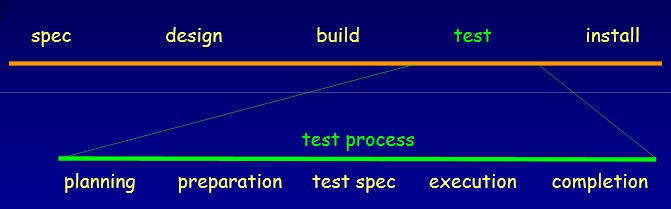
\includegraphics[width=0.7\linewidth]{Tmap1.jpg}

Testing is a process itself in parallel with the development process and has 5 phases.
\subsection{Phase 1: Test Planning and Control}
\begin{itemize*}
    \item Start at requirements phase of system development
    \item Development of master test plan and derived test plans
    \item Under responsibility of test manager
    \item Description of (for each level of detail, system, integration, module, unit)
        \begin{itemize*}
            \item what: objectives, tasks, deliverables
            \item by whom: personnel, responsibilities
            \item with what: infrastructure
            \item in which time: planning
        \end{itemize*}
    \item Risk assessment: what and how thoroughly to test
    \item Control and management during remaining phases
\end{itemize*}

Plan:
\begin{itemize*}
    \item Test Mission/Vision: global, politically oriented, goal of testing for company
    \item Test Strategy
        \begin{itemize*}
            \item High level test approach for company, department
            \item Which levels of testing, techniques for testing, \ldots
            \item For: shared common understanding
        \end{itemize*}
    \item Test approach: Implementation of test strategy for project. Risk assessment, test project goals etc.
    \item Test plan: implementation of test approach: who is doing what and when, with what, what costs, \ldots
\end{itemize*}

\subsection{Phase 2: Preparation}
\begin{itemize*}
    \item Study of test basis (= specification + documentation)
    \item Reviewing of specifications
    \item Check of testability of specifications
    \item Specifications under formal change and configuration control
    \item Division of system into sub-systems which will be separately delivered and tested
\end{itemize*}

\subsection{Phase 3: Test generation (specification)}
\begin{itemize*}
    \item Generation and specification of test cases
    \item Development of infrastructure for test execution
    \item Implementation of test cases on infrastructure (= physical test case design = test script = executable test)
\end{itemize*}

\subsection{Phase 4: Test Execution}
\begin{itemize*}
    \item Testing in phases: completeness checks $\to$ basic functionality test $\to$ full functional testing
    \item Execution: test $\to$ repair $\to$ re-test
    \item Reporting about tests and quality: defects found, what has been and needs to be tested, trends.
\end{itemize*}

\subsection{Phase 5: Completion}
\begin{itemize*}
    \item Final reporting: remaining risks
    \item Preservation of testware for regression or maintenance testing
    \item Evaluation
\end{itemize*}

